\documentclass[11pt,a4paper]{article}
\usepackage[margin=1in]{geometry}
\usepackage{graphicx}
\usepackage{booktabs}
\usepackage{longtable}
\usepackage{float}
\usepackage{hyperref}
\usepackage{amsmath}
\hypersetup{colorlinks=true, linkcolor=blue, urlcolor=blue}
\setlength{\parskip}{0.4em}
\setlength{\parindent}{0pt}
\graphicspath{{assets/}}

\begin{document}

\begin{titlepage}
\centering
{\LARGE 260325\_SpeedEstimation\_Summary\par}
\vspace{1.2cm}
{\Large Comprehensive Internal Report for the SpeedEstimation Project\par}
\vspace{1.0cm}
{\large Repository: /home/chanyoungko/IIT/SpeedEstimation\par}
\vspace{0.6cm}
{\large Date: 2026-03-25\par}
\vfill
{\large This report summarizes the repository structure, input feature generation, preprocessing, model families, training methodology, archive-by-archive experiments, quantitative results, deployment constraints, and real-time feasibility.\par}
\vfill
\end{titlepage}

\tableofcontents
\clearpage

\section{Project Overview}

The repository studies treadmill walking speed estimation from a multi-sensor biomechanics setup. The main target is the left treadmill belt speed. Inputs can include motion capture joint kinematics, IMU measurements, force plate signals, exoskeleton torque, and basic subject information.

The central engineering constraint of this repository is that any final model must remain suitable for real-time inference. That requirement affects not only the neural network itself, but also the whole online path from preprocessing to derived-feature computation and final prediction.

\section{Data and Evaluation Setup}

The main HDF5 dataset is organized in the hierarchy Subject, Condition, Level, and Trial. Milestone2 experiments use subjects from m2\_S001 to m2\_S008. The condition set includes constant-speed trials, acceleration sine trials, incline and decline trials, and stop-and-go trials. The sampling rate is 100Hz.

Most season2 experiments discussed in this report used a single-LOSO setup with m2\_S008 as the held-out test subject. This means the comparisons are valid as internal relative rankings, but they are not yet equivalent to a full LOSO evaluation over all subjects.

The main reported metrics are MAE, RMSE, temporal lag in milliseconds, parameter count, and host latency in milliseconds.

\section{Pipeline Summary}

The overall pipeline is:

\[
\text{raw HDF5 trial data} \rightarrow \text{derived features} \rightarrow \text{sliding windows} \rightarrow \text{normalization} \rightarrow \text{causal model} \rightarrow \text{speed estimate}
\]

The loader generates several derived features on the fly. The dataset module converts trial arrays into sliding windows. The trainer handles scaling, model fitting, validation, testing, and metric export. The comparison script generates evaluation plots and ablation summaries.

An important implementation detail is the trial-level cache, which avoids recomputing derived features for the same trial across repeated fold construction.

\section{Input Features}

\subsection{Feature groups}

The main input groups used in season2 are:

\begin{itemize}
\item motion capture joint kinematics: hip, knee, and ankle angles, plus first and second derivatives, total 18 channels,
\item body-frame IMU signals: 7 channels,
\item IMU-integrated speed prior: 1 channel,
\item model-based COM speed prior: 1 channel,
\item robot torque: 2 channels,
\item GRF and contact signals: 8 channels,
\item subject information: height and weight, 2 channels.
\end{itemize}

\begin{figure}[H]
\centering
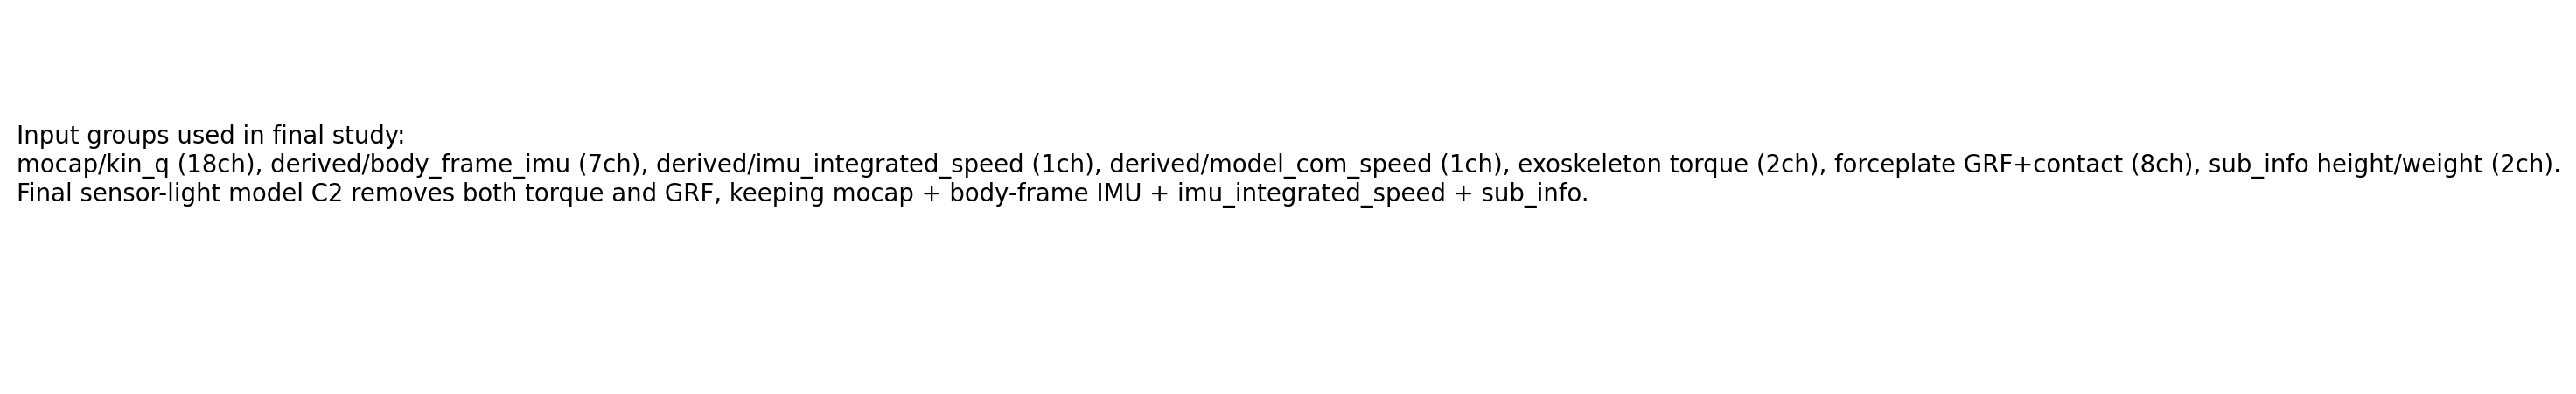
\includegraphics[width=0.95\linewidth]{input_groups_summary.png}
\caption{Input groups used in the final study, including the sensor-light model.}
\end{figure}

The repository does not use common assist level as an input feature. This was checked explicitly and the project rule now forbids adding it in future archives.

\subsection{Body-frame IMU}

One of the most important season2 ideas was converting trunk IMU signals into a body-aligned frame. Instead of reading the raw sensor axes directly, the code reconstructs a local right-forward-up frame and projects linear acceleration and gyroscope signals into that frame.

The most important derived quantity is the overground-like forward acceleration:

\[
\mathrm{forward\_accel\_overground} = a_{\mathrm{body,forward}} + a_{\mathrm{treadmill}}
\]

This gave the model a much more task-aligned inertial signal.

\subsection{IMU-integrated speed}

The IMU-integrated speed feature is not a raw integral of the original IMU. It uses the body-frame forward acceleration, adds treadmill acceleration to create an overground-equivalent signal, then performs leaky integration and causal low-pass filtering.

\[
v_t = \alpha v_{t-1} + a_t \Delta t
\]

Across season2, this became the strongest single physics-inspired prior.

\subsection{Model-based COM speed}

The model-based COM speed feature uses a forward-kinematics approximation from joint angles and pelvis motion, together with GRF-based stance detection, to estimate forward COM speed. This idea was physically appealing, but in practice it was consistently weaker than the IMU-integrated speed prior.

\subsection{Subject information}

Only height and weight were used. These act as anthropometric constants and were never the main source of gain, but they were kept in most final configurations.

\section{Preprocessing and Windowing}

The common season2 setting used:

\begin{itemize}
\item window size 300,
\item training stride 5,
\item inference stride 1,
\item output delay of 5 frames,
\item standard normalization,
\item optional instance normalization inside the model.
\end{itemize}

At 100Hz, a 300-step input window corresponds to about 3 seconds of history, and a 5-frame output delay corresponds to about 50ms ahead prediction.

Later real-time archives also tested window sizes 200, 150, and 120 to improve deployment characteristics.

\section{Model Families}

\subsection{Baseline model}

The baseline model family is a temporal convolutional encoder followed by a GRU head. This design remained strong throughout the project and is the basis of the strongest archive\_2 model.

\subsection{Additional variants}

The following families were explored in season2:

\begin{itemize}
\item attention-enhanced TCN,
\item multiscale TCN plus GRU,
\item causal smoothing TCN plus GRU,
\item observer-style propagated prior plus learned correction,
\item confidence-weighted fusion between learned and physics-based sources.
\end{itemize}

Most structure-only changes did not improve the main baseline.

\subsection{Observer model}

The observer-style model propagated a prior estimate and then added a gated learned correction. It was one of the most paper-motivated ideas in the project. However, the empirical results were weak and often unstable.

\subsection{Fusion model}

The fusion model was the most promising new family. It combined a learned branch with one or more causal priors and estimated source weights from the encoded temporal context. In effect, it learned when to trust the network and when to trust the priors.

\section{Training Methodology}

The common training setup used AdamW, Huber loss, 30 epochs, batch size 128, AMP, cosine scheduling, and early stopping.

Several additional ideas were tested:

\begin{itemize}
\item hard residual skip,
\item delta-target training,
\item prior-alignment regularization,
\item distillation,
\item robustness augmentation by noise and filtering.
\end{itemize}

The overall pattern was clear. Hard residual approaches failed. Delta-target training was safer than hard residual but did not displace the best baseline. Distillation did not provide a reliable benefit. Soft prior alignment and confidence-weighted fusion were the only later ideas that remained meaningfully useful.

\section{Archive-by-Archive Progress}

\subsection{Season1 reference}

Late season1 experiments improved the raw-IMU setup through filtering, augmentation, and test-time tricks. The best confirmed late-season1 number was about MAE 0.0140 in archive\_round8.

\subsection{archive\_1}

archive\_1 introduced the body-frame representation and physics-inspired speed priors. This was the first major shift in representation. It produced the first clear improvement over the late season1 reference.

\subsection{archive\_2}

archive\_2 performed the key ablation study. It directly compared raw IMU formulations, body-frame IMU, IMU-integrated speed, and model-based COM speed. The winner was the combination of body-frame IMU and IMU-integrated speed. This archive produced the strongest absolute baseline in the project.

\subsection{archive\_3}

archive\_3 focused on residual designs. This was the main negative-result archive. Most residual variants collapsed badly and did not remain competitive.

\subsection{archive\_4}

archive\_4 tested delta targets and soft prior losses. This improved substantially over archive\_3 but still did not beat the strong archive\_2 baseline.

\subsection{archive\_5}

archive\_5 explored observer models, fusion, and distillation. Observer models failed. Distillation did not help. Fusion was the only clearly positive new direction.

\subsection{archive\_6}

archive\_6 was the final deployment-oriented archive. It tested:

\begin{itemize}
\item a final accuracy-oriented fusion variant,
\item lightweight real-time variants,
\item sensor-light variants,
\item a tiny-model Pareto point.
\end{itemize}

\begin{figure}[H]
\centering
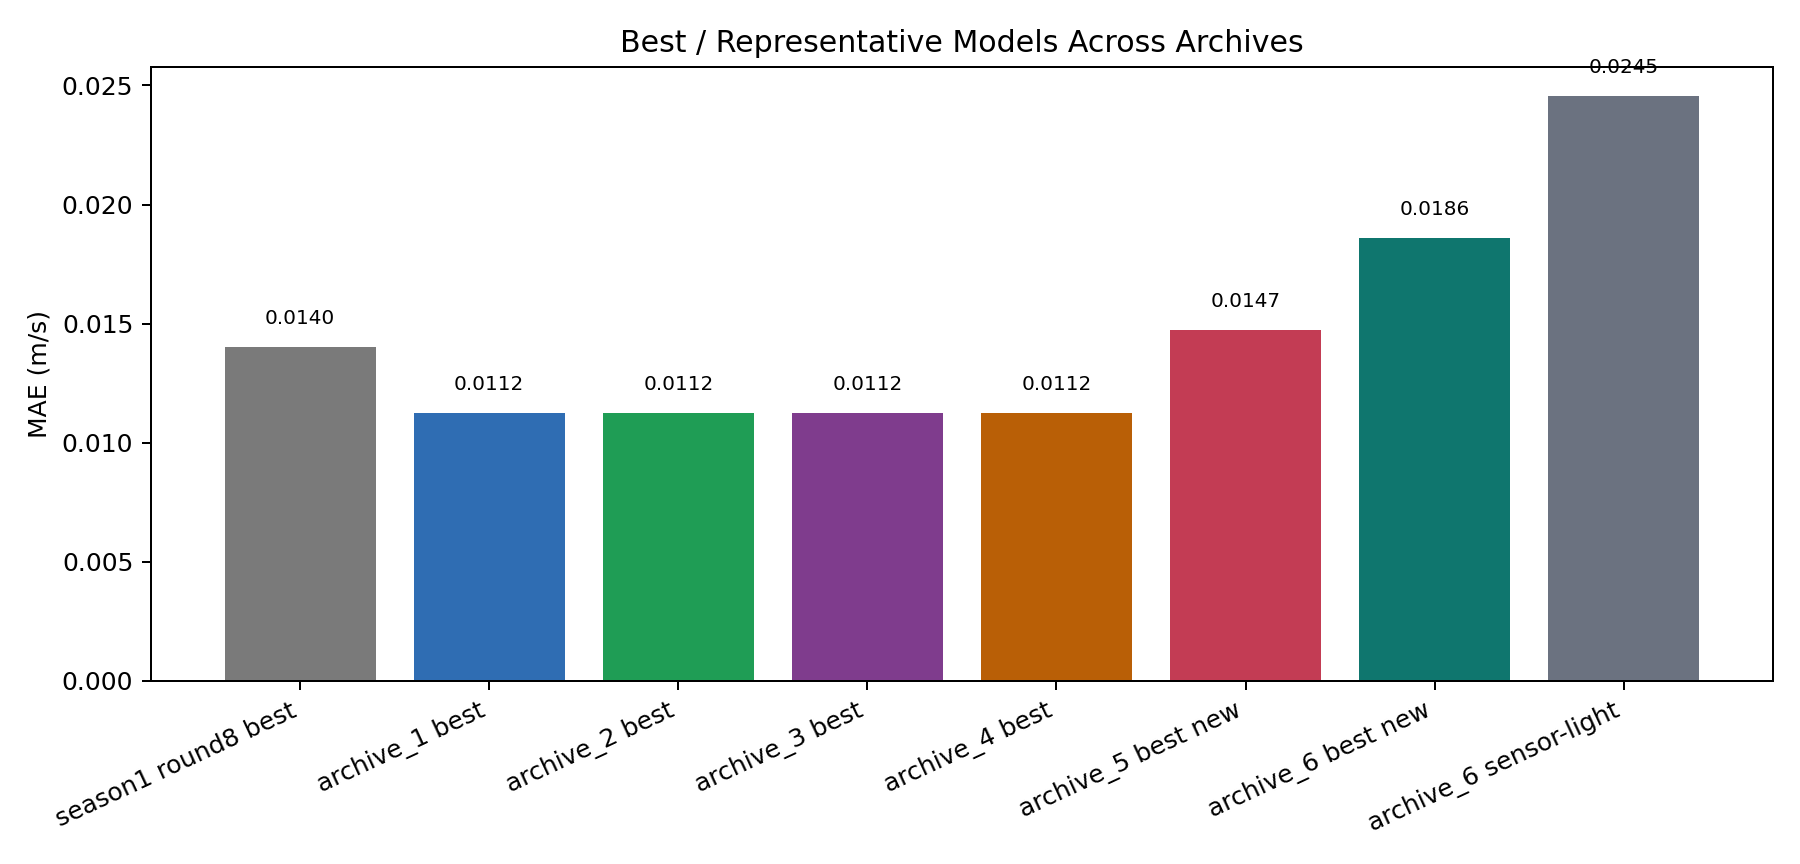
\includegraphics[width=0.98\linewidth]{archive_summary_mae.png}
\caption{Representative MAE values across the project timeline.}
\end{figure}

\section{Key Quantitative Results}

\subsection{Best absolute model}

The strongest absolute result remained the archive\_2 best model based on body-frame IMU plus IMU-integrated speed. Its MAE is about 0.01125 with about 410k parameters.

\subsection{Best new family}

The strongest new family after that baseline was the fusion family. The most representative examples are:

\begin{itemize}
\item archive\_5 fusion with IMU prior, MAE about 0.0147,
\item archive\_6 dual-prior fusion plus soft prior, MAE about 0.0186.
\end{itemize}

\subsection{Deployment-oriented models}

\begin{table}[H]
\centering
\small
\begin{tabular}{lrrrrl}
\toprule
Model & MAE & Params & Latency & Window & Main value \\
\midrule
A5 baseline & 0.0112 & 409793 & 2.4 to 4.1 ms & 300 & best absolute accuracy \\
A5 fusion best new & 0.0147 & 409892 & 2.58 ms & 300 & strongest new model family \\
A6 dual plus soft prior & 0.0186 & 410117 & 2.82 ms & 300 & best final fusion variant \\
A5 real-time fusion & 0.0215 & 143973 & 2.51 ms & 200 & lightweight real-time candidate \\
A6 sensor-light C2 & 0.0245 & 142364 & 2.63 ms & 150 & removes GRF and torque \\
A6 tiny B3 & 0.0403 & 74293 & 2.68 ms & 120 & ultra-light Pareto point \\
\bottomrule
\end{tabular}
\caption{Representative models for accuracy and deployment tradeoffs.}
\end{table}

\begin{figure}[H]
\centering
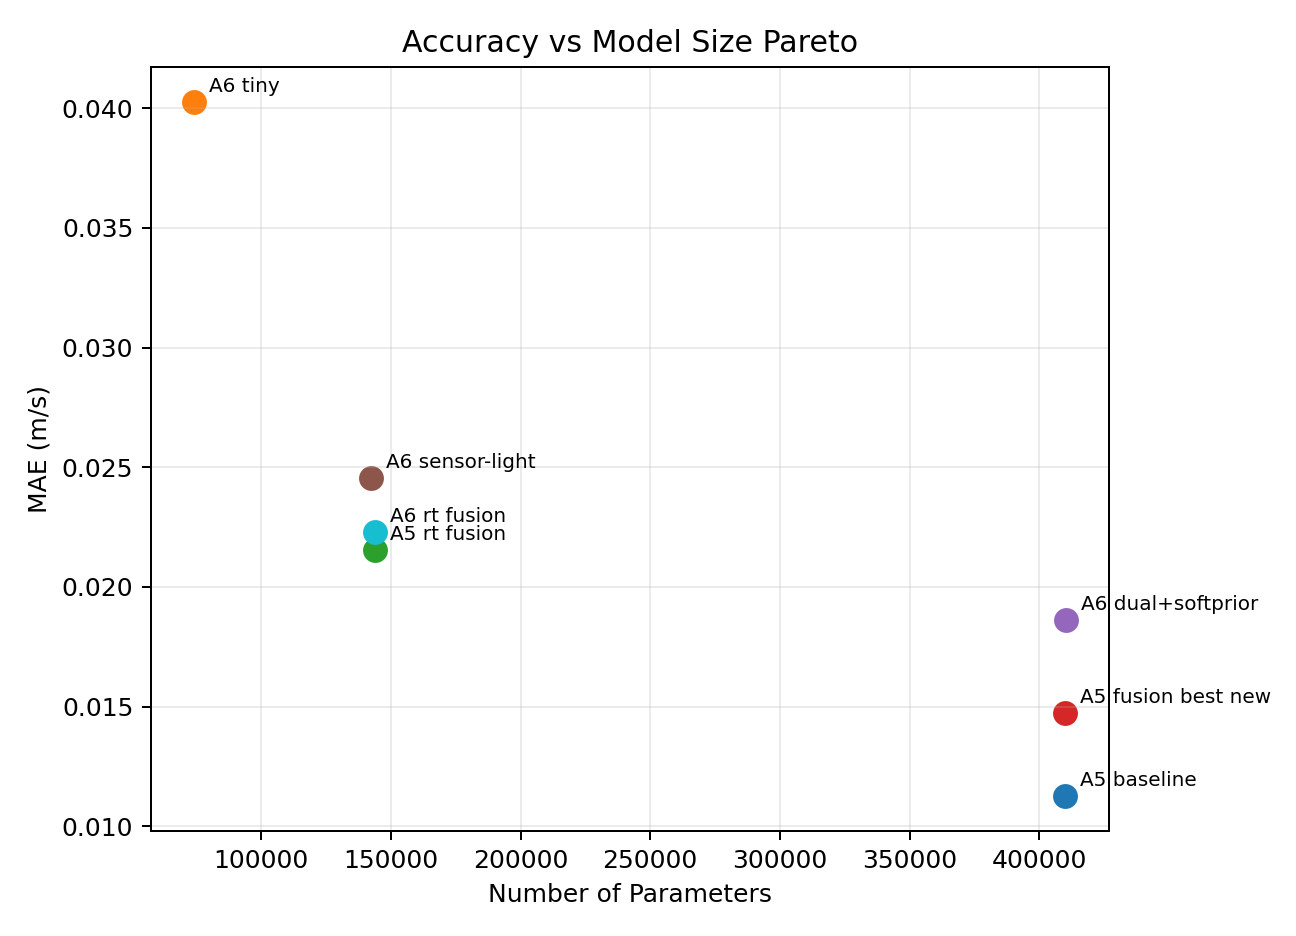
\includegraphics[width=0.82\linewidth]{pareto_params_mae.png}
\caption{Accuracy versus parameter count for representative final models.}
\end{figure}

\section{Qualitative Analysis}

archive\_1 and archive\_2 already contain useful trajectory and condition plots. These plots show that the strongest baseline family tracks the main speed profile well across both constant and dynamic conditions.

\begin{figure}[H]
\centering

\includegraphics[width=0.92\linewidth]{../../compare_result/archive_season2/archive_2/final_comparison_mae.png}
\caption{archive\_2 MAE comparison plot.}
\end{figure}

\begin{figure}[H]
\centering

\includegraphics[width=0.92\linewidth]{../../compare_result/archive_season2/archive_2/final_ablation_delta.png}
\caption{archive\_2 ablation delta plot.}
\end{figure}

\begin{figure}[H]
\centering

\includegraphics[width=0.92\linewidth]{../../compare_result/archive_season2/archive_2/exp_A5_bodyframe_plus_imuint_Test-m2_S008_seed42/exp_A5_bodyframe_plus_imuint_Test-m2_S008_seed42/trajectory.png}
\caption{Trajectory plot of the strongest archive\_2 model.}
\end{figure}

\begin{figure}[H]
\centering

\includegraphics[width=0.92\linewidth]{../../compare_result/archive_season2/archive_1/exp_S2_imu_speed_only_Test-m2_S008_seed42/exp_S2_imu_speed_only_Test-m2_S008_seed42/trajectory.png}
\caption{Trajectory plot of the strongest archive\_1 model.}
\end{figure}

\begin{figure}[H]
\centering
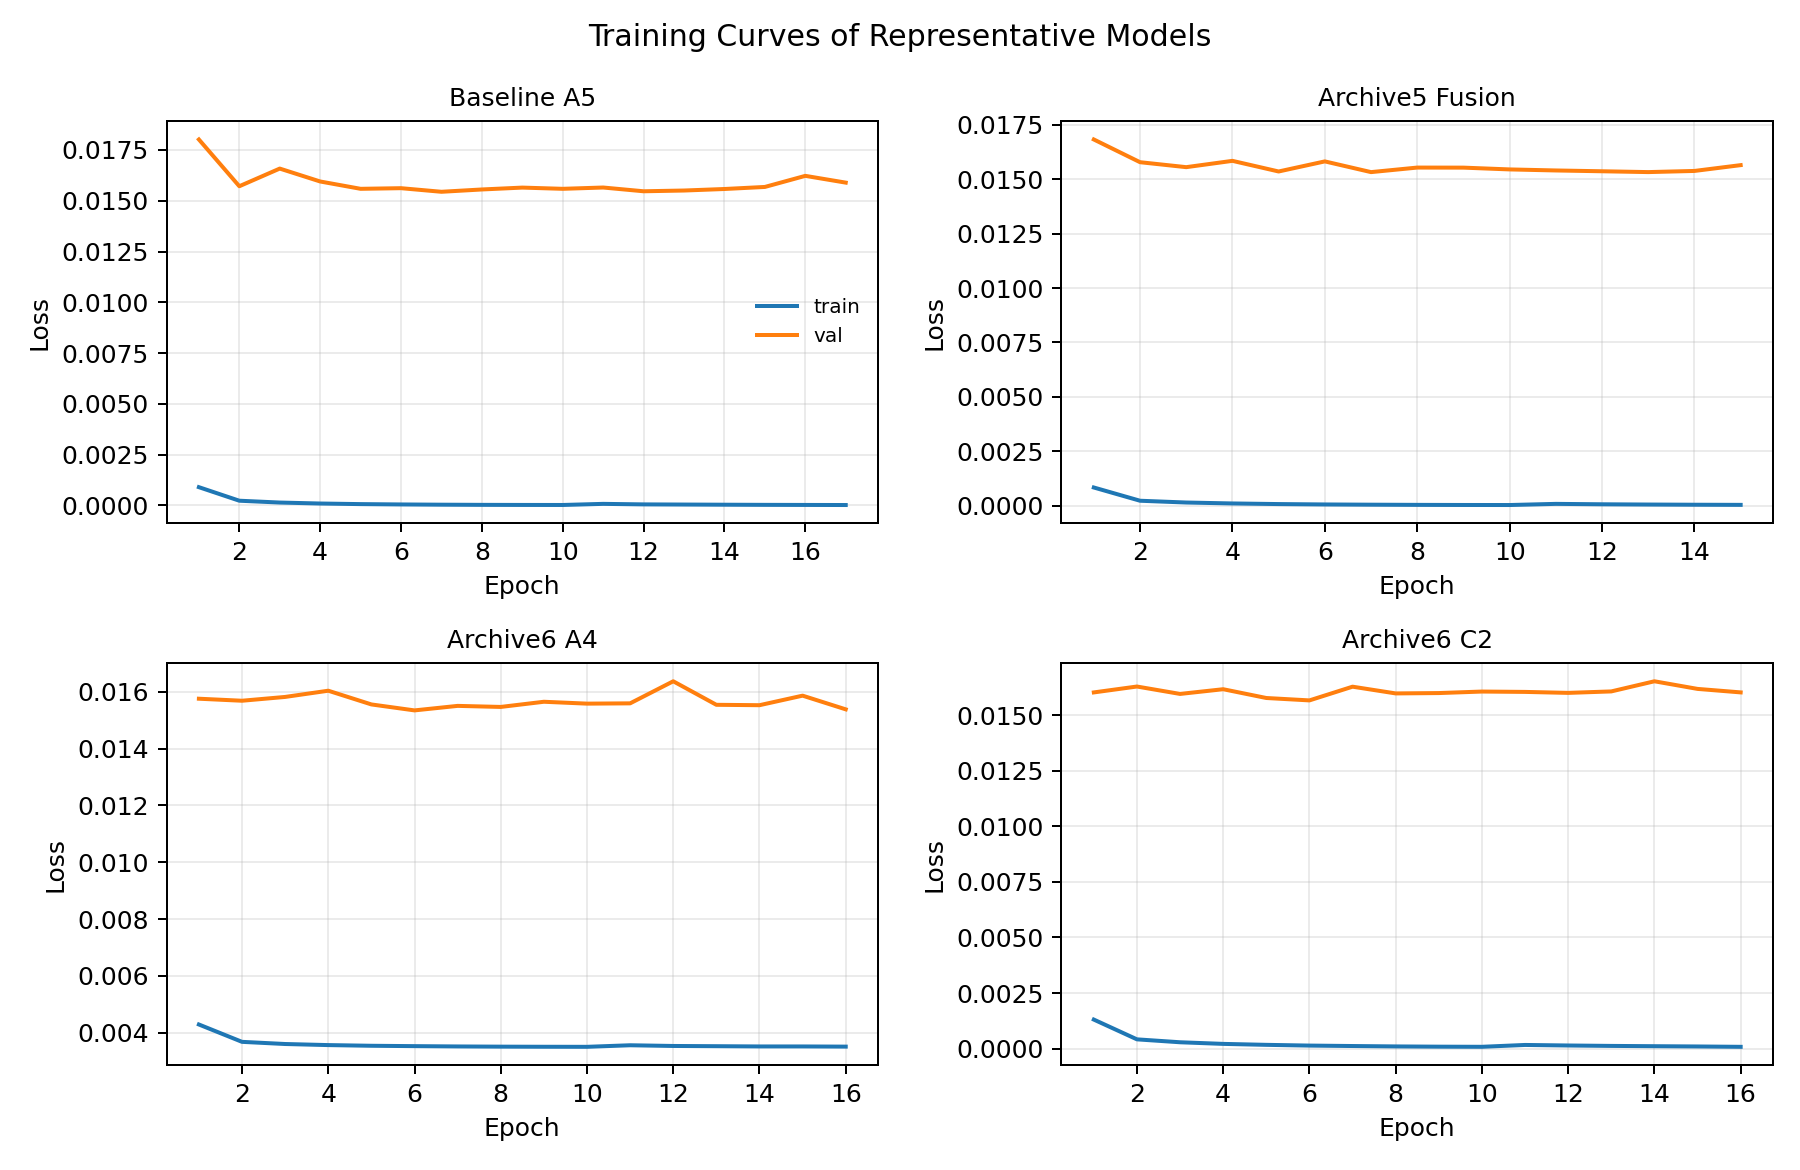
\includegraphics[width=0.95\linewidth]{training_curves_selected.png}
\caption{Training curves of representative baseline, fusion, and sensor-light models.}
\end{figure}

\section{Feature Importance and Interpretation}

The repository currently retains a feature-importance plot from the earlier best-model analysis. While not every season2 archive has an equivalent retained figure, the full season2 outcome strongly supports the same high-level interpretation:

\begin{itemize}
\item body-frame inertial representation is valuable,
\item the IMU-integrated speed prior is the single strongest physics-based cue,
\item the model-based COM speed is interpretable but not dominant,
\item GRF and torque become partially removable when the inertial and kinematic representation is strong enough.
\end{itemize}

\begin{figure}[H]
\centering

\includegraphics[width=0.82\linewidth]{../../experiments/archive_season1/feature_importance_best.png}
\caption{Existing feature-importance visualization retained from the earlier project stage.}
\end{figure}

\section{Real-Time Inference Feasibility}

\subsection{Why the final models are still online-feasible}

The final candidate models remain plausible for real-time use because all important derived features are causal and lightweight. Body-frame IMU requires vector operations and frame projection. IMU-integrated speed requires scalar leaky integration and causal low-pass filtering. Model-based COM speed requires simple kinematic chain calculations and contact logic. None of these steps depends on expensive optimization or future context.

\subsection{Measured model cost}

Measured host latencies are generally in the low millisecond range. The exact latency value varies by run, so small differences should not be over-interpreted. The stable conclusion is that the final candidate models are all in a practical real-time range.

\subsection{Input-buffer memory}

The rolling input buffer is also small:

\begin{itemize}
\item A5 baseline: about 45.6KB,
\item A6 dual plus soft prior: about 46.8KB,
\item A6 C2 sensor-light: about 16.8KB.
\end{itemize}

This means the dominant deployment cost is not the input buffer. It is the model weights and the sensor stack itself.

\subsection{Best deployment choices}

If pure accuracy matters most, the archive\_2 A5 baseline remains the final choice. If deployment matters more, archive\_6 provides stronger candidates:

\begin{itemize}
\item A6 C2 is attractive when torque and GRF are unavailable,
\item A6 B3 is attractive when parameter budget is the main constraint,
\item the archive\_5 and archive\_6 real-time fusion variants are good balanced candidates.
\end{itemize}

\section{What Worked and What Failed}

\subsection{What worked}

\begin{itemize}
\item body-frame IMU,
\item IMU-integrated speed prior,
\item confidence-weighted fusion,
\item sensor-light and parameter-light exploration.
\end{itemize}

\subsection{What failed or remained weak}

\begin{itemize}
\item hard residual skip,
\item observer-style direct propagated correction,
\item distillation,
\item purely structural changes without a stronger representation shift.
\end{itemize}

\section{Final Recommendations}

The strongest overall recommendation is to treat the archive\_2 best model as the accuracy reference and the archive\_6 models as the deployment-oriented reference set.

The most practical shortlist is:

\begin{itemize}
\item archive\_2 A5 for the best absolute accuracy,
\item archive\_5 B1 as the strongest new fusion-family representative,
\item archive\_6 A4 as the best final fusion design,
\item archive\_6 C2 as the best sensor-light model,
\item archive\_6 B3 as the best ultra-light Pareto point.
\end{itemize}

From a paper-writing perspective, the strongest honest contribution is not simply ``the new model beats the old model.'' The stronger story is that body-aligned inertial representation and a causal IMU-based speed prior produce the strongest baseline, and that fusion, sensor reduction, and model-size reduction provide a realistic deployment-oriented contribution without breaking real-time feasibility.

\clearpage
\appendix
\section{Appendix A: Season2 Experiment Table}
\small
\begin{longtable}{r l r r r r}
\caption{Season2 archive experiments and key metrics (single LOSO on m2\_S008).}\\
\toprule
Archive & Experiment & MAE & RMSE & Params & Latency (ms) \\
\midrule
\endfirsthead
\toprule
Archive & Experiment & MAE & RMSE & Params & Latency (ms) \\
\midrule
\endhead
1 & \texttt{baseline\_bodyframe} & 0.0149 & 0.0418 & 409601 & 2.488 \\
1 & \texttt{baseline\_modelbased} & 0.0133 & 0.0382 & 409985 & 2.450 \\
1 & \texttt{exp\_S1\_com\_speed\_only} & 0.0169 & 0.0451 & 409793 & 2.571 \\
1 & \texttt{exp\_S2\_imu\_speed\_only} & 0.0112 & 0.0304 & 409793 & 2.572 \\
1 & \texttt{exp\_S3\_no\_grf} & 0.0285 & 0.0648 & 408449 & 2.593 \\
1 & \texttt{exp\_S4\_no\_raw\_imu} & 0.0203 & 0.0404 & 407585 & 2.378 \\
1 & \texttt{exp\_S5\_residual\_com} & 0.1067 & 0.1413 & 409985 & 2.467 \\
1 & \texttt{exp\_S6\_residual\_imu} & 0.5931 & 0.7902 & 409985 & 2.469 \\
1 & \texttt{exp\_S7\_residual\_com\_only} & 0.0923 & 0.1209 & 409793 & 2.489 \\
2 & \texttt{exp\_A1\_rawimu\_baseline\_repro} & 0.0208 & 0.0489 & 409025 & 2.581 \\
2 & \texttt{exp\_A2\_rawori\_plus\_imuint} & 0.0306 & 0.0646 & 409025 & 2.434 \\
2 & \texttt{exp\_A3\_bodyframe\_imu\_only} & 0.0149 & 0.0418 & 409601 & 2.452 \\
2 & \texttt{exp\_A4\_bodyframe\_plus\_rawvel} & 0.0208 & 0.0492 & 409793 & 2.557 \\
2 & \texttt{exp\_A5\_bodyframe\_plus\_imuint} & 0.0112 & 0.0304 & 409793 & 2.436 \\
2 & \texttt{exp\_B1\_dualphysics\_baseline} & 0.0133 & 0.0382 & 409985 & 2.544 \\
2 & \texttt{exp\_B2\_dualphysics\_multiscale} & 0.0170 & 0.0434 & 1642465 & 7.065 \\
2 & \texttt{exp\_B3\_dualphysics\_causalsmooth} & 0.0377 & 0.0816 & 410337 & 2.592 \\
2 & \texttt{exp\_B4\_dualphysics\_attention} & 0.0264 & 0.0454 & 402978 & 2.376 \\
2 & \texttt{exp\_C1\_dualphysics\_global\_lpf8} & 0.0386 & 0.0769 & 409985 & 2.565 \\
2 & \texttt{exp\_C2\_dualphysics\_pergroup\_noise} & 0.0366 & 0.0778 & 409985 & 2.458 \\
2 & \texttt{exp\_C3\_dualphysics\_lpf\_noise\_combo} & 0.0224 & 0.0515 & 409985 & 2.486 \\
2 & \texttt{exp\_D1\_dualphysics\_longwindow400} & 0.0225 & 0.0498 & 409985 & 2.488 \\
2 & \texttt{exp\_D2\_dualphysics\_shortwindow200} & 0.0184 & 0.0419 & 409985 & 2.460 \\
2 & \texttt{exp\_D3\_dualphysics\_wide\_model} & 0.0156 & 0.0403 & 1618689 & 2.516 \\
3 & \texttt{exp\_A1\_a5\_repro} & 0.0112 & 0.0304 & 409793 & 2.656 \\
3 & \texttt{exp\_A2\_imuint\_residual} & 0.6155 & 0.8403 & 409793 & 2.594 \\
3 & \texttt{exp\_A3\_dualphysics\_imuint\_residual} & 0.5931 & 0.7902 & 409985 & 2.757 \\
3 & \texttt{exp\_A4\_dualphysics\_modelcom\_residual} & 0.1067 & 0.1413 & 409985 & 2.596 \\
3 & \texttt{exp\_B1\_rt\_win200\_residual} & 0.6733 & 0.9016 & 409793 & 2.520 \\
3 & \texttt{exp\_B2\_rt\_win150\_residual} & 0.6746 & 0.8976 & 409793 & 2.551 \\
3 & \texttt{exp\_B3\_rt\_win200\_small\_residual} & 0.7786 & 1.0423 & 232465 & 2.477 \\
3 & \texttt{exp\_B4\_rt\_win150\_small\_residual} & 0.7985 & 1.0444 & 232465 & 2.674 \\
3 & \texttt{exp\_C1\_no\_grf\_residual} & 0.5596 & 0.7510 & 408257 & 2.500 \\
3 & \texttt{exp\_C2\_no\_torque\_residual} & 0.5876 & 0.7783 & 409409 & 2.600 \\
3 & \texttt{exp\_C3\_tcnonly\_win150\_residual} & 0.7051 & 0.9265 & 232169 & 2.341 \\
4 & \texttt{exp\_A1\_a5\_repro} & 0.0112 & 0.0304 & 409793 & 2.656 \\
4 & \texttt{exp\_A2\_delta\_imuint} & 0.1844 & 0.2430 & 409793 & 3.489 \\
4 & \texttt{exp\_A3\_delta\_dual\_imuint} & 0.1865 & 0.2537 & 409985 & 2.578 \\
4 & \texttt{exp\_A4\_delta\_dual\_modelcom} & 0.0382 & 0.0515 & 409985 & 2.548 \\
4 & \texttt{exp\_B1\_softprior\_imuint\_light} & 0.0282 & 0.0434 & 409793 & 4.067 \\
4 & \texttt{exp\_B2\_softprior\_imuint\_strong} & 0.0959 & 0.1272 & 409793 & 2.461 \\
4 & \texttt{exp\_B3\_softprior\_dual\_imuint} & 0.0437 & 0.0668 & 409985 & 2.538 \\
4 & \texttt{exp\_C1\_delta\_imuint\_win200} & 0.2002 & 0.2686 & 409793 & 2.767 \\
4 & \texttt{exp\_C2\_delta\_imuint\_win150} & 0.2003 & 0.2692 & 409793 & 2.592 \\
4 & \texttt{exp\_C3\_delta\_imuint\_win150\_small} & 0.2245 & 0.3000 & 232465 & 2.502 \\
5 & \texttt{exp\_S2A5\_A1\_a5\_repro} & 0.0112 & 0.0304 & 409793 & 2.388 \\
5 & \texttt{exp\_S2A5\_A2\_observer\_imuint} & 0.6350 & 0.8396 & 409859 & 2.486 \\
5 & \texttt{exp\_S2A5\_A3\_observer\_imuint\_prop} & 0.6752 & 0.8878 & 409860 & 2.561 \\
5 & \texttt{exp\_S2A5\_A4\_observer\_dual\_imuint} & 0.6930 & 0.9313 & 410052 & 2.538 \\
5 & \texttt{exp\_S2A5\_A5\_observer\_dual\_modelcom} & 0.0898 & 0.1169 & 410052 & 2.637 \\
5 & \texttt{exp\_S2A5\_B1\_fusion\_imuint} & 0.0147 & 0.0396 & 409892 & 2.583 \\
5 & \texttt{exp\_S2A5\_B2\_fusion\_dual} & 0.0256 & 0.0434 & 410117 & 2.714 \\
5 & \texttt{exp\_S2A5\_B3\_fusion\_imuint\_rt} & 0.0223 & 0.0436 & 143804 & 2.530 \\
5 & \texttt{exp\_S2A5\_B4\_fusion\_dual\_rt} & 0.0215 & 0.0469 & 143973 & 2.511 \\
5 & \texttt{exp\_S2A5\_C1\_distill\_small\_a5} & 0.0386 & 0.0590 & 143729 & 2.354 \\
5 & \texttt{exp\_S2A5\_C2\_distill\_observer\_imuint} & 0.8748 & 1.1500 & 143780 & 2.522 \\
5 & \texttt{exp\_S2A5\_C3\_distill\_fusion\_dual} & 0.0333 & 0.0556 & 143973 & 2.523 \\
6 & \texttt{exp\_S2A6\_A1\_a5\_repro} & 0.0112 & 0.0304 & 409793 & 4.092 \\
6 & \texttt{exp\_S2A6\_A2\_fusion\_imuint\_repro} & 0.0147 & 0.0396 & 409892 & 4.077 \\
6 & \texttt{exp\_S2A6\_A3\_fusion\_imuint\_softprior} & 0.0294 & 0.0618 & 409892 & 4.313 \\
6 & \texttt{exp\_S2A6\_A4\_fusion\_dual\_softprior} & 0.0186 & 0.0402 & 410117 & 2.816 \\
6 & \texttt{exp\_S2A6\_B1\_fusion\_dual\_rt200} & 0.0215 & 0.0469 & 143973 & 2.594 \\
6 & \texttt{exp\_S2A6\_B2\_fusion\_imuint\_rt150} & 0.0223 & 0.0436 & 143804 & 2.534 \\
6 & \texttt{exp\_S2A6\_B3\_fusion\_dual\_tiny120} & 0.0403 & 0.0750 & 74293 & 2.681 \\
6 & \texttt{exp\_S2A6\_C1\_fusion\_imuint\_nogrf} & 0.0360 & 0.0713 & 142652 & 4.413 \\
6 & \texttt{exp\_S2A6\_C2\_fusion\_imuint\_nogrf\_notorque} & 0.0245 & 0.0536 & 142364 & 2.627 \\
6 & \texttt{exp\_S2A6\_C3\_fusion\_dual\_nogrf\_notorque} & 0.0274 & 0.0553 & 142533 & 2.639 \\
\bottomrule
\end{longtable}

\end{document}
